\chapter{tracer\_decay}

\section{Purpose}

To demonstrate that \telemac{2D} can model the transport of non-conservative
tracer in a flow when coupled with \waqtel.

%\section{Approach}
\section{Description}
The validation is processed with a hypothetical one-dimensional flow with
constant velocity (0.03~m/s) and constant depth (10~m).

A 11,400~m long and 50~m wide channel with a flat bottom is considered.
%
\section{Computational options}
%
\subsection{Mesh}
%
The triangular mesh is composed of 2,850 triangular elements (element size
of triangles = 40~m along the channel bank and 10~m along the channel width)
and 1,716 nodes (see Figure \ref{fig:tracer_decay:mesh} with a zoom close to
the left boundary in Figure \ref{fig:tracer_decay:mesh_zoomed}).

\begin{figure}[H]
\centering
  \includegraphicsmaybe{[width=.8\textwidth]}{../img/mesh.png}
\caption{Mesh}\label{fig:tracer_decay:mesh}
\end{figure}

\begin{figure}[H]
\centering
  \includegraphicsmaybe{[width=.8\textwidth]}{../img/mesh_zoomed.png}
\caption{Zoom of the mesh close to the left boundary}\label{fig:tracer_decay:mesh_zoomed}
\end{figure}

\subsection{Physical parameters}

Initial condition:
\begin{itemize}
\item The concentration of the tracer is 30~mg/l at the left boundary
nodes and 0~mg/l at all other nodes (as shown in Figures
\ref{fig:tracer_decay:tracer_t0_zoomed} and \ref{fig:tracer_decay:tracer_t0}),
\item Constant velocity 0.03~m/s,
\item Constant water height 10~m.
\end{itemize}

\begin{figure}[H]
\centering
  \includegraphicsmaybe{[width=.8\textwidth]}{../img/tracer_t0_zoomed.png}
\caption{Initial state of tracer zoomed close to the left boundary}\label{fig:tracer_decay:tracer_t0_zoomed}
\end{figure}

\begin{figure}[H]
\centering
  \includegraphicsmaybe{[width=.8\textwidth]}{../img/tracer_t0.png}
\caption{Initial state of tracer}\label{fig:tracer_decay:tracer_t0}
\end{figure}

Boundary conditions:
\begin{itemize}
\item Left inlet boundary:
\begin{itemize}
\item Constant velocity of 0.03~m/s,
\item Constant tracer concentration of 30~mg/l for first 6 hours, 0~mg/l after,
\end{itemize}
\item Right outlet boundary:
\begin{itemize}
\item Constant velocity of -0.03~m/s,
\item Free tracer concentration,
\end{itemize}
\item Lateral boundaries: solid smooth boundary.
\end{itemize}

Bottom:
\begin{itemize}
\item Flat bottom without friction.
\end{itemize}

Parameters for non-conservative tracers:
\begin{itemize}
\item Number of tracer: 1,
\item Coefficient for diffusion of tracers: 30~m$^2$/s,
\item Decay rate as a law for bacterial degradation:
0; 1.0/day; 2.0/day.
\end{itemize}

\subsection{General parameters}

The time step is 100~s for a simulated period of 6~days (= 518,400~s).

\subsection{Numerical parameters}

Tracer:
\begin{itemize}
\item Advection of tracer: method of characteristics,
%\item Solver for diffusion of tracer: conjugate gradient method,
\item Accuracy for diffusion of tracers: 10$^{-10}$.
\end{itemize}

Flow and velocity:
\begin{itemize}
  \item No diffusion,
  \item No advection.
\end{itemize}

\section{Results}

The tracer concentration time series of analysis and simulation at $x$ = 2,000~m
are compared (see Figure \ref{fig:tracer_decay:sol_anal}).
Visually the solution produced by \telemac{2D} shows very good
agreement with the exact solution.
For 6 days of simulation duration, when $K_d$ = 0 or $K_d$ = 1/day, the model
peak time is 5 minutes earlier than the exact peak time;
and for $K_d$ = 2/day, the time difference is less than 2 minutes.

\begin{figure}[H]
\centering
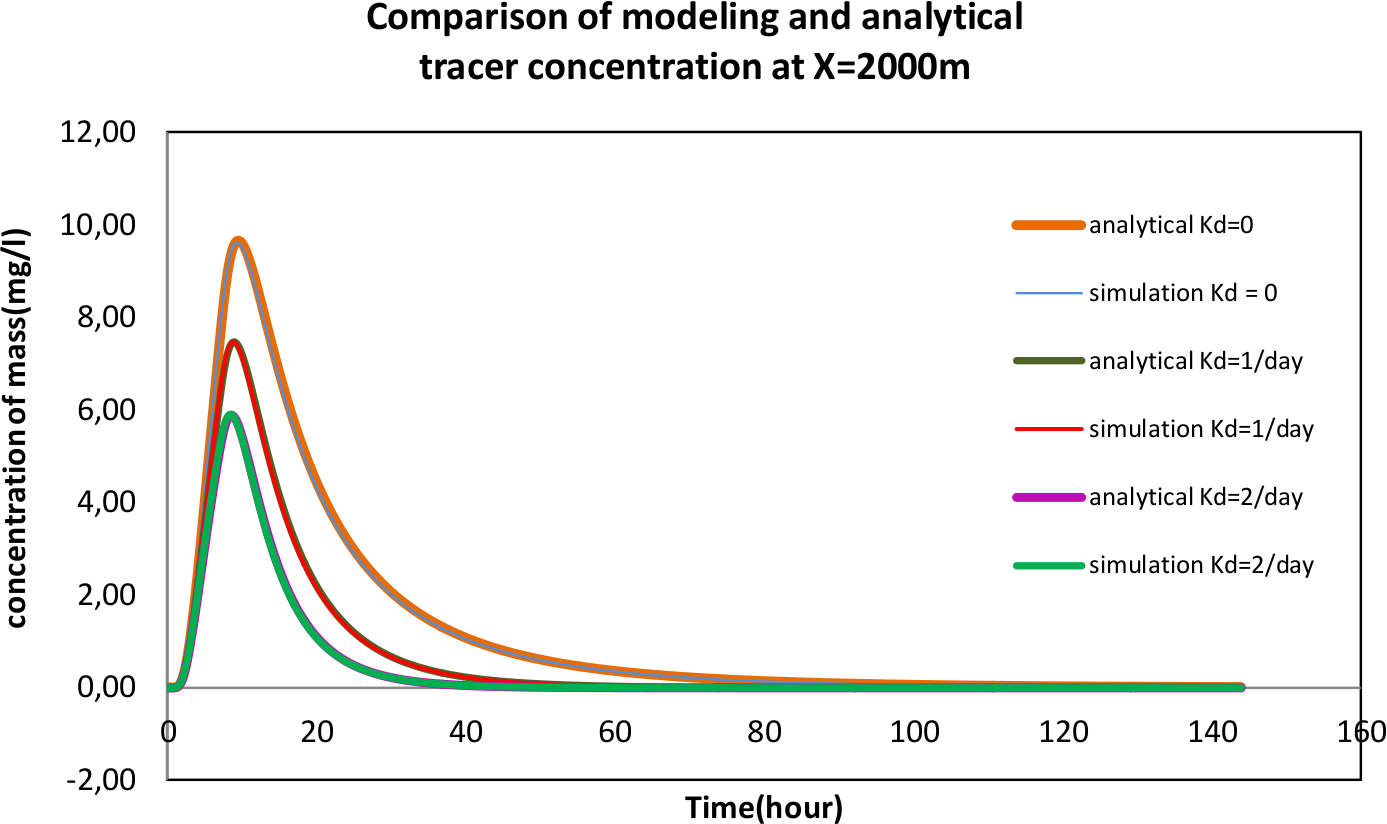
\includegraphics[width=.6\textwidth]{img/sol_anal}
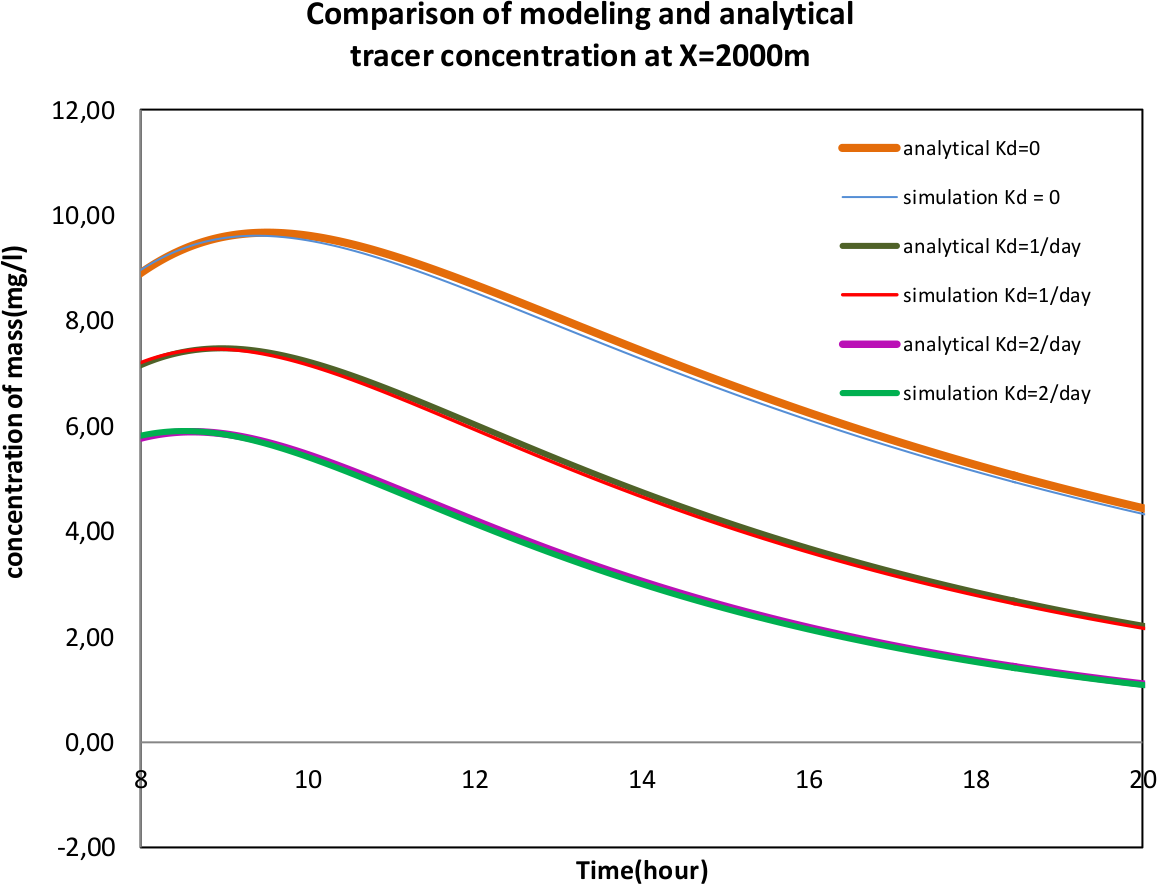
\includegraphics[width=.6\textwidth]{img/sol_anal_zoomed}
\caption{Comparison between analytical solution and \telemac{2D} solution for non-conservative tracer transport}\label{fig:tracer_decay:sol_anal}
\end{figure}

\section{Conclusion}
\telemac{2D} reproduces accurately the transport of non-conservative tracers
when coupled with \waqtel.
